\documentclass[]{LASPreport}


\newcommand{\SubSystem}{ADCS}
\newcommand{\SERnumber}{Thruster Unit Test}
\newcommand{\subject}{Unit Test Results for Thruster Simulation Model}
\newcommand{\status}{Initial Test Results}
\newcommand{\preparer}{S. Piggott}
\newcommand{\summary}{
   This is a report documenting the results of the thruster model unit test created for 
   the AVS Basilisk Simulation as part of the EMM project. }


\begin{document}


\makeCover


%
%	enter the revision documentation here
%	to add more lines, copy the table entry and the \hline, and paste after the current entry.
%
\pagestyle{empty}
{\renewcommand{\arraystretch}{2}
\noindent
\begin{longtable}{|p{0.5in}|p{4.5in}|p{1.14in}|}
\hline
{\bfseries Rev}: & {\bfseries Change Description} & {\bfseries By} \\
\hline
Draft & Initial Revision & S. Piggott \\
\hline

\end{longtable}
}

\newpage
\setcounter{page}{1}
\pagestyle{fancy}

\tableofcontents
~\\ \hrule ~\\

%\begin{figure}[htb]
%	\centerline{
%	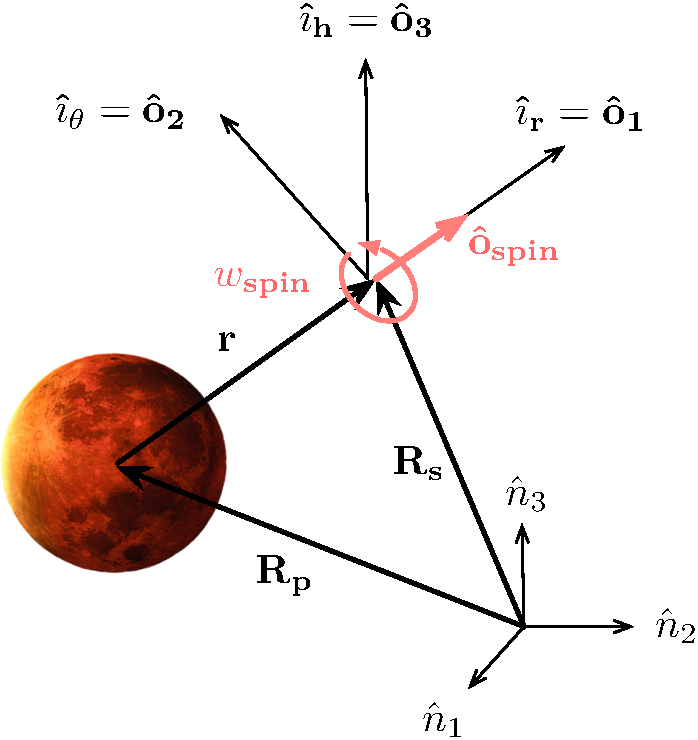
\includegraphics[]{Figures/Fig1}
%	}
%	\caption{Sample Figure Inclusion.}
%	\label{fig:Fig1}
%\end{figure}

\section{Introduction}
The Thruster model in the AVS Basilisk simulation is used to emulate the effect 
of a vehicle's thrusters on the overall system.  Its primary use is to generate 
realistic forces/torques on the vehicle structure and body.  This is 
accomplished by apply a force at a specified location/direction in the body and 
using the current vehicle center of mass to calculate the resultant torque.  
Each individual thruster in a given model has its own ramp-up/ramp-down profile 
specified as part of its initialization data and it follows those profiles during 
start-up and shutdown.

The thruster model also contains a mechanism that is used to change the current 
vehicle mass properties as the thruster fires propellant overboard.  This model 
uses the thruster ISP (specific impulse, also specified with configuration data) 
to calculate how much mass is being removed during a given thruster firing and 
decrements the mass properties included in the thruster linearly as a function 
of mass.  

The model can be configured according to the user's wishes, but the following 
rules of thumb should probably be respected unless you are incredibly confident 
in your own smartness.
\begin{enumerate}
\item{The internal simulation dynamics step time should be less than or equal 
     to the thruster ramp-up/ramp-down time steps}
\item{The internal simulation dynamics step time should be less than or equal to 
     the desired thruster discretization level}
\item{The internal simulation dynamics step time should be less than one-tenth 
    of the expected minimum allowable thruster firing duration}
\end{enumerate}


\section{Test Design}
The unit test for the thruster\_dynamics module is located in:\\

\noindent
{\tt SimCode/dynamics/Thrusters/UnitTest/ThrusterDynamicsUnitTest.py \\
\\

\noindent This unit test is designed to functionally test the simulation model 
outputs as well as get complete code path coverage.  The test design is broken 
up into several parts:\\
\begin{enumerate}
\item{Thruster Force Orientation: The output forces/torques from the simulation 
  are checked to ensure that their values/directions are correct per the 
  simulation inputs.}
\item{Instantaneous On/Off Factor: The thrusters are fired with an 
  instantaneous ramp to ensure that the firing is correct depending on the 
  simulation dynamics rate.  This includes propellant depletion.}
\item{Short Instantaneous Firing: A "short" firing that still respects the 
  rules of thumb above is fired to ensure that it is still correct enough.}
\item{Ramp On/Ramp Off Firing: A set of ramps are set for the thruster to ensure 
  that the ramp configurationis respected during a ramped firing.}
\end{enumerate}


\section{Test Results}
\begin{enumerate}
\item{Thruster Force Orientation:}
\item{Instantaneous On/Off Factor:}
\item{Short Instantaneous Firing:}
\item{Ramp On/Ramp Off Firing:}
\end{enumerate}

\section{Test Coverage}
The method coverage for all of the methods included in the spice\_interface 
module are tabulated in Table~\ref{tab:cov_met}

\begin{table}[htbp]
    \caption{Test Analysis Results}
   \label{tab:cov_met}
        \centering \fontsize{10}{10}\selectfont
   \begin{tabular}{c | r | r | r} % Column formatting, 
      \hline
      Method Name    & Unit Test Coverage (\%) & Runtime Self (\%) & Runtime Children (\%) \\
      \hline
      SelfInit & 100.0 & 0.0 & 0.0 \\
      CrossInit & 100.0 & 0.0 & 0.0 \\
      AddThruster & 100.0 & 0.0 & 0.0 \\
      UpdateState & 100.0 & 0.0 & 0.0 \\
      WriteOutputMessages & 100.0 & 0.0 & 0.0 \\
      ReadInputs & 100.0 & 0.0 & 0.0 \\
      ConfigureThrustRequests & 100.0 & 0.0 & 0.0 \\
      ComputeDynamics & 100.0 & 0.0 & 0.0 \\
      ComputeThrusterFire & 100.0 & 0.0 & 0.0 \\
      ComputeThrusterShut & 100.0 & 0.0 & 0.0 \\
      updateMassProperties & 100.0 & 0.0 & 0.0 \\
      \hline
   \end{tabular}
\end{table}

For all of the methods in the spice\_interface modules, the code coverage 
percentage is 100\% which meets our test requirements.  

\section{Conclusions}

\end{document}
